\documentclass[conference, a4paper]{IEEEtran}
\usepackage[utf8]{inputenc}
\usepackage[spanish]{babel}
\usepackage{cite}
\usepackage{amsmath,amssymb,amsfonts}
\usepackage{graphicx}
\usepackage{hyperref}
\usepackage{tabularx}
\usepackage{float}
\usepackage{booktabs}

\begin{document}

\title{SocioUnido: Ecosistema SaaS inteligente para la gesti\'on descentralizada y control de accesos offline en instituciones deportivas}

\author{\IEEEauthorblockN{Felipe Santino Ascencio, Lautaro Gabriel Ghosn, Mart\'in Guerrero, Axel Zielonka}
\IEEEauthorblockA{\textit{Facultad de Ingenier\'ia} \\
\textit{Universidad de Buenos Aires (FIUBA)}\\
Buenos Aires, Argentina \\
\{fascencio, lghosn, mguerrero, azielonka\}@fi.uba.ar}
}

\maketitle

\begin{abstract}
El presente art\'iculo documenta el dise\~no, desarrollo e implementaci\'on de SocioUnido, una plataforma integral \textit{Software as a Service} (SaaS) bajo un modelo E2E (\textit{Enterprise-to-Enterprise}) orientada a modernizar la gesti\'on administrativa y el control de accesos en clubes deportivos argentinos. La soluci\'on aborda de manera directa tres ineficiencias cr\'iticas del sector: la morosidad societaria silenciosa, el fraude en accesos por pr\'estamo de credenciales y la subutilizaci\'on de activos institucionales. Tecnol\'ogicamente, la plataforma propone un ecosistema modular de vanguardia que incluye: un control de accesos perimetral descentralizado basado en algoritmos TOTP (\textit{Time-Based One-Time Password}) capaz de operar 100\% \textit{offline} para superar el colapso sistem\'atico de redes en estadios; un asistente conversacional cognitivo (BotIn) soportado por procesamiento de lenguaje natural (PLN) para la autogesti\'on sin fricci\'on; y un motor anal\'itico para la prevenci\'on proactiva del abandono (\textit{churn}). Validado mediante metodolog\'ias \`agiles, auditor\'ias DevSecOps y testing automatizado con agentes de IA, SocioUnido demuestra ser una herramienta robusta y escalable que promueve el saneamiento financiero institucional y la inclusi\'on tecnol\'ogica.
\end{abstract}

\begin{IEEEkeywords}
SaaS, Control de Accesos Offline, TOTP, Machine Learning, DevSecOps, Gesti\'on Deportiva, QA Automatizado.
\end{IEEEkeywords}

% ==========================================
\section{Introducci\'on}
% ==========================================

\subsection{Contexto y motivaci\'on}
Las asociaciones civiles deportivas sin fines de lucro en la Rep\'ublica Argentina constituyen pilares fundamentales para la cohesi\'on social, la contenci\'on comunitaria y la promoci\'on de actividades culturales y recreativas. A diferencia del modelo societario de propiedad privada imperante en otras latitudes, el club deportivo argentino opera tradicionalmente bajo un esquema democr\'atico donde el socio es el verdadero propietario y gestor de la instituci\'on. No obstante, a pesar de su incalculable valor sociocultural, la inmensa mayor\'ia de estas entidades de tama\~no mediano y peque\~no ---desde los clubes de las categor\'ias de ascenso del \'area metropolitana de Buenos Aires hasta las ligas regionales del interior del pa\'is--- enfrentan un escenario de marcada vulnerabilidad financiera, profundizado por la subsistencia de pr\'acticas de gesti\'on administrativa marcadamente tradicionales y reactivas.

Hist\'oricamente, la adopci\'on de herramientas tecnol\'ogicas avanzadas ha sido un privilegio exclusivo de las escasas corporaciones deportivas que de forma sistem\'atica acceden a los recursos de la \'elite profesional de primera divisi\'on. Para las instituciones del ascenso y del interior, la digitalizaci\'on de sus operaciones suele limitarse a la implementaci\'on de planillas de c\'alculo manuales aisladas, sistemas de base de datos desactualizados o simples sistemas de registro de transacciones gen\'ericos de tipo reactivo, conocidos t\'ecnicamente como sistemas \textit{CRUD} b\'asicos (crear, leer, actualizar y borrar). Esta brecha tecnol\'ogica genera un aislamiento operativo que restringe la capacidad de las dirigencias para automatizar procesos administrativos rutinarios, optimizar la recaudaci\'on de cuotas, prevenir fugas de capital y garantizar la seguridad perimetral de sus instalaciones durante eventos de concurrencia masiva.

Frente a esta realidad, el presente trabajo documenta el dise\~no, desarrollo e implementaci\'on de \textbf{SocioUnido}, un ecosistema de \textit{software} modular concebido bajo un modelo de \textit{software} como servicio (\textit{SaaS}) y marca blanca, espec\'ificamente dimensionado para resolver las demandas operativas reales de las instituciones deportivas argentinas. El proyecto no se concibe como una simple herramienta contable digital, sino como una plataforma inteligente, descentralizada y proactiva de inteligencia de negocios y ciberseguridad aplicada al saneamiento financiero y la inclusi\'on tecnol\'ogica institucional.

\subsection{Planteamiento del problema y faltante en el sector}
El an\'alisis de dominio realizado sobre la gesti\'on operativa de los clubes deportivos en Argentina permiti\'o identificar tres ineficiencias cr\'iticas de car\'acter silencioso que impactan directamente sobre su rentabilidad econ\'omica y su sostenibilidad institucional:

\begin{enumerate}
    \item \textbf{La morosidad societaria silenciosa:} Debido a la desconexi\'on existente entre las actividades deportivas de los socios, los registros administrativos y los medios de pago disponibles, las instituciones deportivas sufren una p\'erdida constante de ingresos por cuotas sociales impagas. La falta de canales digitales inmediatos y la dependencia de cobros manuales presenciales en tesorer\'ias centralizadas fomentan un comportamiento de olvido por parte de los usuarios. Al no contar con alertas proactivas ni motores capaces de anticipar la morosidad o la intenci\'on de baja societaria, los clubes act\'uan reactivamente una vez que la deuda se ha consolidado y la p\'erdida del socio es irreversible.
    \item \textbf{El fraude en el control de accesos por duplicaci\'on o pr\'estamo de credenciales f\'isicas:} En eventos masivos, la utilizaci\'on de credenciales impresas pl\'asticas con c\'odigos de barras est\'aticos o sistemas magn\'eticos heredados propicia el pr\'estamo de carnets entre socios activos y personas no autorizadas. Esta duplicidad de accesos genera no solo una severa fuga de recaudaci\'on por entradas no vendidas, sino tambi\'en una grave vulnerabilidad de seguridad l\'ogica y f\'isica en los puntos de control del estadio. La soluci\'on tradicional exige conectividad permanente de banda ancha de alta velocidad en los molinetes perimetrales para validar la validez de los c\'odigos contra la base de datos central en la nube. Sin embargo, en escenarios masivos, la saturaci\'on por radiofrecuencia y la ca\'ida recurrente de las redes de telefon\'ia celular m\'ovil imposibilitan la validaci\'on en tiempo real (\textit{online}), obligando en muchas ocasiones al personal de control a liberar los ingresos para evitar desmanes f\'isicos, validando involuntariamente accesos fraudulentos o de socios morosos.
    \item \textbf{La subutilizaci\'on de instalaciones comunes, disciplinas y activos deportivos rentables:} Gran parte de los clubes poseen instalaciones ociosas (como canchas auxiliares, quinchos, salones o predios de entrenamiento) e infraestructura de disciplinas deportivas infrautilizadas debido a la ausencia de un canal centralizado de reservas. Los socios deben acudir presencialmente o comunicarse telef\'onicamente en horarios acotados para consultar disponibilidad, lo que desincentiva el consumo interno y reduce las fuentes de financiamiento alternativas de la instituci\'on.
\end{enumerate}

SocioUnido nace con el firme prop\'osito de mitigar estas problem\'aticas de ra\'iz, integrando en una \'unica plataforma la gesti\'on administrativa y social proactiva, la prevenci\'on anal\'itica de la morosidad y un sistema de control de accesos seguro y descentralizado capaz de validar ingresos masivos de forma 100\% fuera de l\'inea (\textit{offline}).

\subsection{Objetivos del Trabajo Profesional}
\subsubsection{Objetivo general}
Dise\~nar, desarrollar y validar un ecosistema de \textit{software} integral y adaptativo de marca blanca que centralice la administraci\'on de clubes deportivos, optimice la retenci\'on y fidelizaci\'on societaria mediante mecanismos cognitivos y predictivos, y blinde el per\'imetro de las instalaciones mediante una soluci\'on criptogr\'afica de control de accesos descentralizada y tolerante a fallos de conectividad.

\subsubsection{Objetivos espec\'ificos}
Para alcanzar el objetivo general, se definen las siguientes metas t\'ecnicas y metodol\'ogicas:
\begin{itemize}
    \item Implementar una arquitectura perimetral y distribuida de microservicios resiliente, escalable y cibersegura, orquestada mediante contenedores y centralizada bajo un portal de enlace de aplicaciones (\textit{API gateway}) unificado.
    \item Desarrollar una aplicaci\'on web progresiva (\textit{PWA}) adaptativa para el socio, compatible con dispositivos m\'oviles de bajos recursos, que centralice su credencial digital, la reserva de espacios, la inscripci\'on a disciplinas y el flujo transaccional de pagos.
    \item Dise\~nar y validar un algoritmo de control de accesos inteligente basado en c\'odigos criptogr\'aficos de un solo uso basados en tiempo (\textit{TOTP}), que permita la validaci\'on instant\'anea del estado de pago e identidad del socio sin requerir conectividad de red (\textit{offline}) en los dispositivos de escaneo del club.
    \item Construir un asistente transaccional conversacional interactivo cognitivo (asistente ``BotIn''), con procesamiento de lenguaje natural (\textit{PLN}), para reducir la fricci\'on transaccional administrativa a cero.
    \item Dise\~nar y desarrollar una plataforma web de administraci\'on centralizada que permita a las autoridades del club digitalizar de forma integral los procesos institucionales, automatizar la facturaci\'on y cobranza de cuotas sociales, y gestionar de manera eficiente las disciplinas deportivas y los activos compartidos.
    \item Validar metodol\'ogicamente el proceso de ingenier\'ia de \textit{software} utilizando el marco \'agil Scrum y certificar la calidad, ciberseguridad e interoperabilidad del c\'odigo fuente de forma continua mediante el an\'alisis est\'atico y un agente aut\'onomo de aseguramiento de calidad (\textit{QA}) basado en inteligencia artificial.
\end{itemize}

\subsection{Articulaci\'on e integraci\'on de conocimientos acad\'emicos de la carrera}
El dise\~no y materializaci\'on del ecosistema SocioUnido no constituye una actividad de desarrollo tecnol\'ogico aislada, sino la s\'intesis pr\'actica y la convergencia multidisciplinar de los conocimientos te\'oricos adquiridos a lo largo de toda la trayectoria acad\'emica en la Facultad de Ingenier\'ia de la Universidad de Buenos Aires. La resoluci\'on de los desaf\'ios del dominio deportivo y de infraestructura requiri\'o articular de forma sin\'ergica conocimientos de \'areas diversas de la inform\'atica y de la formaci\'on general del ingeniero:

\begin{itemize}
    \item \textbf{Ciencias b\'asicas e infraestructura f\'isica}: Los fundamentos de electromagnetismo, atenuaci\'on de ondas de radiofrecuencia y saturaci\'on de espectro analizados en las asignaturas de F\'isica y F\'isica para Inform\'atica proveyeron el sustento cient\'ifico para predecir el colapso de las antenas celulares en los estadios de f\'utbol ante altas densidades de usuarios. Esta base f\'isica justific\'o de manera irrefutable la necesidad de dise\~nar un sistema de control de ingresos descentralizado y desacoplado de la red en la nube.
    \item \textbf{Matem\'aticas avanzadas y criptograf\'ia}: Las teor\'ias de aritm\'etica modular, funciones unidireccionales y transformaciones matriciales estructuradas en \'Algebra y \'Algebra Lineal permitieron desarrollar y robustecer el algoritmo criptogr\'afico del sistema de accesos \textit{offline} mediante semillas \textit{TOTP} e implementar firmas digitales con claves sim\'etricas seguras e infalsificables.
    \item \textbf{Ingenier\'ia de software, dise\~no y arquitectura distribuidos}: Los conceptos de encapsulamiento, modularidad y dise\~no orientado a objetos (entre muchos otros) provistos por Paradigmas de Programaci\'on y Taller de Programaci\'on guiaron la construcci\'on de un c\'odigo fuente limpio y mantenible. Por su parte, Base de Datos aport\'o el marco te\'orico del modelo relacional, control de transacciones concurrentes complejas y optimizaci\'on de consultas SQL en PostgreSQL. Redes y Sistemas Distribuidos I fueron la base t\'ecnica para dise\~nar la topolog\'ia de microservicios, la tolerancia a fallos y la comunicaci\'on interservicio as\'incrona.
    \item \textbf{Ciberseguridad y defensa profunda}: La aplicaci\'on de los lineamientos de an\'alisis de vulnerabilidades, sanitizaci\'on de entradas, prevenci\'on de inyecciones y control estricto de roles de acceso mediante JSON Web Tokens (\textit{JWT}) provienen directamente del Taller de Seguridad Inform\'atica, construyendo una infraestructura segura contra ataques perimetrales.
    \item \textbf{Emprendedurismo, \'etica y contexto profesional}: El desarrollo de un producto m\'inimo viable comercializable, el estudio macrocontextual bajo la metodolog\'ia de las 5 C, el an\'alisis microcontextual de las 4 P, el seguimiento de m\'etricas \textit{SaaS} y la gesti\'on \'agil \textit{Scrum} se forjaron de manera directa sobre las bases conceptuales y procedimentales adquiridas a lo largo de un trayecto de cuatro materias clave: ingenier\'ia del software I, ingenier\'ia del software II, empresas de base tecnol\'ogica I y empresas de base tecnol\'ogica II. Estas asignaturas proveyeron el andamiaje metodol\'ogico para estructurar tanto el ciclo de vida del producto de software como su estrategia de viabilidad y comercializaci\'on en el mercado real.
\end{itemize}

% ==========================================
\section{Estado del Arte}
% ==========================================

\subsection{El paradigma tradicional de gesti\'on deportiva y el \textit{status quo}}
El mercado de soluciones inform\'aticas destinadas a la administraci\'on de instituciones deportivas en la Rep\'ublica Argentina se ha caracterizado hist\'oricamente por un profundo conservadurismo metodol\'ogico y tecnol\'ogico. Las herramientas utilizadas por la inmensa mayor\'ia de las comisiones directivas de clubes de mediana y peque\~na envergadura evidencian un rezago estructural frente a las transformaciones digitales observadas en otras industrias de servicios masivos. El denominado \textit{status quo} operativo se asienta sobre tres metodolog\'ias tradicionales que limitan severamente el control y el crecimiento institucional:

\begin{enumerate}
    \item \textbf{Gesti\'on anal\'ogica y descentralizada}: El uso de planillas impresas f\'isicas en papel para el control diario de las instalaciones, actas manuales para el registro de los libros de socios y la conciliaci\'on contable presencial en ventanillas de tesorer\'ia centralizadas. Este enfoque no solo es propenso a errores humanos sistem\'aticos y p\'erdidas f\'isicas de informaci\'on, sino que demanda una asignaci\'on desproporcionada de horas-hombre en tareas administrativas rutinarias de escaso valor agregado.
    \item \textbf{Soporte en herramientas ofim\'aticas gen\'ericas}: El empleo de planillas de c\'alculo (como Microsoft Excel) operadas de forma aislada por los coordinadores de cada disciplina deportiva. La fragmentaci\'on de los datos impide consolidar un padr\'on \'unico de socios, lo que genera inconsistencias cr\'iticas de informaci\'on (como socios dados de baja que contin\'uan asistiendo a actividades, o viceversa) y anula cualquier capacidad de an\'alisis financiero global en tiempo real.
    \item \textbf{Credenciales de identificaci\'on vulnerables}: La emisi\'on de carnets de pl\'astico f\'isicos basados en tecnolog\'ia de cloruro de polivinilo (\textit{PVC}) con c\'odigos de barras est\'aticos o bandas magn\'eticas heredadas. Estos soportes f\'isicos presentan una alta susceptibilidad al desgaste material, la p\'erdida y, fundamentalmente, la falsificaci\'on o pr\'estamo no autorizado. Esta pr\'actica facilita el acceso de personas con cuotas sociales inactivas, consolidando una morosidad silenciosa y exponiendo la seguridad f\'isica y l\'ogica del club durante eventos de alta concurrencia.
\end{enumerate}

Las pocas instituciones que han implementado sistemas de software locales suelen depender de arquitecturas monol\'iticas locales instaladas en computadoras f\'isicas dentro de las sedes. Estas soluciones exigen una inversi\'on inicial significativa en infraestructura de servidores, sistemas de refrigeraci\'on y copias de seguridad manuales, adem\'as de someter al club a altos costos fijos de mantenimiento t\'ecnico y soporte especializado, lo cual resulta econ\'omicamente inviable para las finanzas de las asociaciones civiles de las categor\'ias de ascenso.

\subsection{An\'alisis cr\'itico de los competidores actuales (caso de referencia: Global.fan)}
Para evaluar la validez t\'ecnica y comercial de SocioUnido en el \'ambito de la ingenier\'ia de software aplicada, resulta indispensable contrastar su propuesta de valor frente a las plataformas de gesti\'on deportiva que dominan el mercado del f\'utbol argentino profesional. El principal caso de referencia local es la plataforma Global.fan, considerada el competidor m\'as representativo de la industria.

El an\'alisis de arquitectura y alcance funcional de estos sistemas comerciales revela limitaciones estructurales cr\'iticas desde la perspectiva de la resiliencia tecnol\'ogica y el valor proactivo del software:

\begin{itemize}
    \item \textbf{Naturaleza reactiva de la informaci\'on (sistemas \textit{CRUD} b\'asicos)}: Los competidores del mercado operan esencialmente como bases de datos est\'aticas basadas en un esquema de creaci\'on, lectura, actualizaci\'on y borrado (\textit{CRUD}). Estos sistemas dependen exclusivamente de la proactividad del usuario administrador o del socio para registrar un dato o gatillar una consulta. Carecen por completo de capas anal\'iticas inteligentes que procesen los flujos de datos hist\'oricos para anticipar comportamientos, limitando la toma de decisiones a reportes hist\'oricos emitidos de manera posterior al hecho consumado (\textit{ex post}).
    \item \textbf{Gesti\'on de morosidad pasiva}: Ante la falta de pago de la cuota social, los sistemas vigentes se limitan a generar un listado est\'atico de morosos. La instituci\'on deportiva debe iniciar manualmente campa\~nas de cobranza tard\'ias sobre usuarios que ya se encuentran desvinculados emocional y financieramente del club. No existen mecanismos preventivos que detecten de forma temprana el riesgo latente de abandono (\textit{churn rate}), cuando la probabilidad de recuperaci\'on del socio y del capital es estad\'isticamente superior.
    \item \textbf{Absoluta dependencia de conectividad perimetral}: Los sistemas din\'amicos de acceso digital implementados por competidores comerciales utilizan c\'odigos \textit{QR} variables que se actualizan de forma constante en la aplicaci\'on del usuario. No obstante, para validar la legitimidad de dicho c\'odigo en las puertas de acceso al estadio, el dispositivo lector o molinete perimetral debe realizar una petici\'on de red (\textit{online}) en tiempo real contra los servidores centrales de la plataforma en la nube. En escenarios de aglomeraci\'on masiva, el colapso sistem\'atico de las celdas de telefon\'ia m\'ovil de cuarta y quinta generaci\'on (4G/5G) impide la comunicaci\'on de red, bloqueando los puntos de escaneo. Esto obliga a la dirigencia deportiva a liberar las puertas por motivos de seguridad civil, anulando la eficacia del sistema de accesos y posibilitando el ingreso de personas no autorizadas o morosas.
    \item \textbf{Aislamiento funcional e interfaces cerradas}: Los sistemas comerciales obligan al socio a descargar aplicaciones nativas pesadas, registrar nuevas cuentas, recordar contrase\~nas adicionales y navegar por plataformas ajenas a sus h\'abitos digitales diarios. Esta fricci\'on en la experiencia de usuario incrementa la tasa de deserci\'on en los flujos de autogesti\'on y pago de cuotas. Asimismo, sus arquitecturas cerradas impiden la interoperabilidad con canales de mensajer\'ia masiva o asistentes conversacionales externos, centralizando la atenci\'on en oficinas f\'isicas presenciales con horarios restringidos.
    \item \textbf{Enfoque comercial sesgado a la \'elite deportiva}: Las plataformas existentes basan su modelo de negocio en la captaci\'on agresiva de los clubes de primera divisi\'on de gran envergadura institucional. La complejidad operativa de sus despliegues de hardware propietario en estadios y las altas tarifas de configuraci\'on inicial (\textit{setup fees}) margina por completo a los clubes del ascenso metropolitano, el ascenso federal y las ligas regionales del interior, profundizando la brecha tecnol\'ogica y de seguridad en el f\'utbol local.
\end{itemize}

\subsection{Ejes de innovaci\'on y disrupci\'on tecnol\'ogica de SocioUnido}
SocioUnido rompe disruptivamente con el estado de la t\'ecnica al introducir un ecosistema de ingenier\'ia de software proactivo, descentralizado y cognitivo. La plataforma no opera como un mero registro pasivo del estado actual del club deportivo, sino que se anticipa a los eventos financieros y operativos mediante la aplicaci\'on de conceptos que redefinen los est\'andares de la industria local. 

El car\'acter innovador y de vanguardia de la soluci\'on se consolida sobre cuatro ejes de alta ingenier\'ia inform\'atica:

\subsubsection{1. Control de accesos descentralizado y tolerante a fallos de red (\textit{smart access offline})}
La disrupci\'on fundamental en materia de ciberseguridad perimetral es la eliminaci\'on absoluta de la dependencia de conectividad de red durante la validaci\'on de ingresos. El m\'odulo de acceso inteligente de SocioUnido implementa un algoritmo criptogr\'afico basado en contrase\~nas de un solo uso basadas en tiempo (\textit{TOTP}, por sus siglas en ingl\'es, \textit{time-based one-time password}), estructurado de la siguiente forma:

\begin{itemize}
    \item \textbf{Generaci\'on aislada en la interfaz del usuario}: La aplicaci\'on web progresiva (\textit{PWA}) del socio genera un c\'odigo \textit{QR} din\'amico que encripta de forma segura una semilla \'unica de identidad y un sello de tiempo. Este proceso matem\'atico se ejecuta localmente en el dispositivo celular del socio sin consumir datos m\'oviles, permitiendo su correcto funcionamiento en escenarios de bloqueo total de red o incluso con el dispositivo en modo avi\'on.
    \item \textbf{Validaci\'on perimetral desacoplada}: El personal de control, utilizando la aplicaci\'on operativa del club instalada en terminales m\'oviles est\'andar, escanea el c\'odigo \textit{QR}. 
    \item \textbf{Mitigaci\'on del fraude mediante protocolos \textit{anti-replay}}: Para impedir la duplicaci\'on de accesos o el pr\'estamo de carnets mediante capturas de pantalla, cada c\'odigo \textit{QR} posee una validez f\'isica estricta. Adicionalmente, el microservicio de acceso de SocioUnido interact\'ua con una cach\'e distribuida en memoria (implementada mediante \textit{Redis}) que almacena y rechaza de manera instant\'anea cualquier intento de reingreso que presente un token ya procesado dentro de la ventana de tiempo activa.
\end{itemize}

\subsubsection{2. Control anal\'itico y proactivo de la morosidad}
A diferencia de los sistemas tradicionales que operan de manera pasiva y tard\'ia, SocioUnido introduce un enfoque anal\'itico y proactivo para la contenci\'on de la morosidad societaria. La plataforma integra un m\'odulo especializado de inteligencia de negocios que procesa de manera continua la informaci\'on de pagos y asistencias del club:

\begin{itemize}
    \item \textbf{Monitoreo automatizado de comportamiento}: El subsistema analiza de manera regular el historial de pagos y el registro f\'isico de accesos del socio. Esto permite identificar de forma autom\'atica patrones de inactividad o retrasos incipientes en el pago de la cuota social, alertando a la administraci\'on antes de que la deuda se consolide cr\'iticamente.
    \item \textbf{Tableros de control proactivos}: A trav\'es del panel web centralizado, las autoridades del club visualizan m\'etricas clave de salud financiera y alertas parametrizadas. Esto permite segmentar al padr\'on de socios seg\'un su nivel de regularidad, facilitando la toma de decisiones basada en datos reales de uso y recaudaci\'on.
    \item \textbf{Campa\~nas autom\'aticas de regularizaci\'on}: Una vez detectada una desviaci\'on en el comportamiento de pago o asistencia, el sistema permite disparar de forma proactiva recordatorios y facilidades transaccionales a trav\'es de canales digitales integrados, reduciendo dr\'asticamente la tasa de abandono de los socios mediante gestiones oportunas.
\end{itemize}

\subsubsection{3. Interacci\'on cognitiva sin fricci\'on: asistente conversacional (BotIn)}
Para superar la tasa de rebote asociada a la descarga e instalaci\'on de aplicaciones nativas complejas en poblaciones deportivas heterog\'eneas, SocioUnido incorpora a su ecosistema un robot conversacional (\textit{bot}) inteligente denominado BotIn, desarrollado sobre la API oficial de Telegram:

\begin{itemize}
    \item \textbf{Procesamiento de lenguaje natural sin rigidez}: El microservicio conversacional utiliza arquitecturas avanzadas de orquestaci\'on cognitiva (como \textit{LangChain}) para comprender el lenguaje cotidiano, coloquial e informal de los socios, superando los r\'igidos esquemas jer\'arquicos de botones de las opciones num\'ericas tradicionales.
    \item \textbf{Orquestaci\'on y cobro din\'amico}: Cuando un socio interact\'ua con el bot (por ejemplo, enviando mensajes como ``Hola, quiero pagar las cuotas que debo'' o ``¿qu\'e canchas hay libres esta tarde?''), el motor reconoce la intenci\'on del usuario (\textit{intent recognition}), extrae los par\'ametros contextuales, consulta en tiempo real el microservicio de gesti\'on contable central y devuelve de manera inmediata un enlace din\'amico de pago integrado con la pasarela transaccional de Mercado Pago, o bien confirma una reserva. Esto reduce la fricci\'on operativa a cero y digitaliza transacciones complejas en segundos desde el canal de comunicaci\'on nativo del usuario.
\end{itemize}

\subsubsection{4. Arquitectura adaptativa de marca blanca para la democratizaci\'on del f\'utbol regional}
El dise\~no arquitect\'onico definitivo de SocioUnido se rige por un principio de adaptabilidad est\'etica y econ\'omica enfocado en dotar a las comisiones directivas de las herramientas que tradicionalmente pertenecieron a los clubes de \'elite:

\begin{itemize}
    \item \textbf{Infraestructura el\'astica en la nube}: Al desplegar la plataforma bajo un modelo \textit{SaaS} multiinquilino (\textit{multi-tenant}) distribuido mediante contenedores y unificado por un portal de enlace de aplicaciones de alto rendimiento (\textit{KrakenD API gateway}), se suprime por completo la necesidad de inversiones iniciales en hardware local o mantenimiento especializado por parte del club deportivo.
    \item \textbf{Marca blanca visualmente neutra y adaptativa}: Para posibilitar la comercializaci\'on masiva del \textit{software} de forma transparente a m\'ultiples instituciones deportivas clientes sin generar sesgos, rivalidades institucionales o fricciones crom\'aticas, SocioUnido adopta un dise\~no visual base estrictamente acrom\'atico (escala de grises neutros). Las interfaces se personalizan y adaptan din\'amicamente mediante hojas de estilo din\'amicas que inyectan los colores corporativos, escudos e identidad institucional de cada club una vez consolidada la suscripci\'on, garantizando un posicionamiento corporativo \'optimo para cada cliente. 
\end{itemize}

% ==========================================
\section{Metodolog\'ia aplicada}
% ==========================================

\subsection{El marco de desarrollo incremental y adaptativo}
La complejidad del ecosistema modular de \textit{SocioUnido} exigi\'o la adopci\'on de una metodolog\'ia de trabajo que garantizara un ciclo de vida de desarrollo de \textit{software} altamente estructurado, auditable y capaz de adaptarse din\'amicamente a los requerimientos t\'ecnicos identificados en el an\'alisis del dominio deportivo argentino. En consonancia con lo establecido por el reglamento, el proyecto se rigi\'o bajo un enfoque iterativo e incremental basado en el marco de trabajo \'agil \textit{Scrum}. Este paradigma metodol\'ogico permiti\'o fragmentar un alcance tecnol\'ogico masivo en incrementos funcionales de valor integrados de forma continua, asegurando que la arquitectura del sistema se mantuviera estable y operable a lo largo de las diversas fases del proyecto.

\subsection{Evoluci\'on y transiciones metodol\'ogicas a lo largo de las 37 semanas}
El ciclo de vida del Trabajo Profesional se extendi\'o a lo largo de un per\'iodo neto de 37 semanas cronol\'ogicas. Sin embargo, la din\'amica del trabajo en equipo y la naturaleza de las tareas acad\'emicas y t\'ecnicas obligaron a realizar transiciones metodol\'ogicas estrat\'egicas, abandonando la linealidad del marco \textit{Scrum} en aquellas fases donde su aplicaci\'on resultaba ineficiente o contraproducente para los objetivos espec\'ificos de ingenier\'ia :

\begin{enumerate}
    \item \textbf{Fase 1: Ideaci\'on, viabilidad y anteproyecto (semanas 1 a 12)}: Durante este per\'iodo inicial, el equipo no aplic\'o el marco de trabajo \textit{Scrum} debido a que el esfuerzo se centr\'o en la exploraci\'on del mercado deportivo, la aplicaci\'on de los marcos anal\'iticos de las 5 C y las 4 P para la evaluaci\'on y descarte de las 13 ideas preliminares de negocio, y el dise\~no de la topolog\'ia preliminar de servicios bajo el modelo de arquitectura C4. La din\'amica de trabajo se rigi\'o por jornadas as\'incronas de investigaci\'on comercial, reuniones semanales de debate y la posterior redacci\'on y entrega del documento de anteproyecto formal.
    \item \textbf{Fase 2: Desarrollo del producto m\'inimo viable bajo Scrum (semanas 13 a 25)}: Esta fase de m\'axima intensidad de desarrollo y codificaci\'on del \textit{software} se gobern\'o de forma estricta por el marco \'agil \textit{Scrum} a lo largo de un ciclo cerrado de trece \textit{sprints} de una semana de duraci\'on cada uno. La cadencia semanal fue elegida para acelerar los ciclos de retroalimentaci\'on interna, permitiendo que al cierre de cada iteraci\'on el equipo dispusiera de un incremento funcional del sistema completamente verificado y desplegado en los entornos de pruebas previas a producci\'on (\textit{staging}).
    \item \textbf{Fase 3: Refinaci\'on, validaci\'on final y cierre (semanas 26 a 37)}: Tras congelar el c\'odigo del producto m\'inimo viable (\textit{MVP}), el equipo abandon\'o de forma consciente el marco \textit{Scrum} para adoptar un esquema de trabajo sumamente flexible basado en incidentes (\textit{issue-driven}) y tableros visuales \textit{Kanban}. Esta transici\'on permiti\'o canalizar de manera eficiente las correcciones de errores (\textit{bugs}) surgidas de las pruebas cualitativas de usuario, aplicar las recomendaciones est\'eticasla, instrumentar la auditor\'ia metodol\'ogica de calidad final y preparar el material de soporte para la defensa oral acad\'emica ante el jurado examinador.
\end{enumerate}

\subsection{Distribuci\'on definitiva de roles y especializaci\'on del equipo de ingenier\'ia}
Para blindar la ejecuci\'on del Trabajo Profesional, la estructura organizativa de \textit{SocioUnido} se fundament\'o en la asignaci\'on de responsabilidades principales y \'areas de soberan\'ia (\textit{ownership}). Si bien los cuatro integrantes del equipo se involucraron activamente de forma transversal en todas las fases del ciclo de vida del \textit{software}, la designaci\'on de un l\'ider especializado por \'area garantiz\'o que cada componente contara con un control de calidad y auditor\'ia interna rigurosa antes de su fusi\'on a la rama principal de c\'odigo.

Al contrastar la ejecuci\'on final con lo planificado originalmente en la propuesta de anteproyecto, se produjo un cambio de roles entre dos de los integrantes del equipo, justificado por la especializaci\'on t\'ecnica y la optimizaci\'on de los flujos de trabajo :

\begin{itemize}
    \item \textbf{Ascencio, Felipe Santino}: Se desempe\~n\'o como responsable de control de calidad (\textit{QA}), documentaci\'on t\'ecnica, desarrollo de negocio y preventa. Lider\'o la planificaci\'on y ejecuci\'on de las bater\'ias de pruebas funcionales y de aceptaci\'on, la definici\'on metodol\'ogica de los criterios de calidad del proceso, la redacci\'on de los documentos t\'ecnicos y el dise\~no de los simuladores interactivos de retorno de inversi\'on para la validaci\'on comercial. 
    \item \textbf{Ghosn, Lautaro Gabriel}: Ejerci\'o el rol de responsable de arquitectura, producto, bases de datos e integraciones del sistema. Tuvo a su cargo el dise\~no y mantenimiento de la topolog\'ia distribuida de microservicios, el modelado relacional e incremental de las bases de datos en la nube, el dise\~no e instrumentaci\'on de las firmas y contratos de las interfaces de programaci\'on de aplicaciones (\textit{APIs}) y la priorizaci\'on del Product Backlog general.
    \item \textbf{Guerrero, Mart\'in}: Asumi\'o el rol de responsable de la capa l\'ogica de servidor (\textit{backend}), inteligencia artificial y relaciones institucionales sectoriales. Martín asumi\'o estas responsabilidades para centralizar con \'exito la implementaci\'on f\'isica de los microservicios en Python y FastAPI, la l\'ogica de seguridad criptogr\'afica del servidor y la orquestaci\'on as\'incrona del asistente conversacional (BotIn) sobre la API de Telegram.
    \item \textbf{Zielonka, Axel}: Asumi\'o las funciones de responsable de interfaces de usuario (\textit{front-end}), experiencia/interfaz de usuario (\textit{UX/UI}) e identidad de marca, ejerciendo adicionalmente el rol fundamental de \textit{scrum master} durante la Fase 2 del desarrollo. Axel lider\'o de forma destacada el desarrollo integral del panel web de administraci\'on web, la maquetaci\'on responsiva de las aplicaciones web progresivas (\textit{PWA}) para socios y empleados de control, el dise\~no de prototipos de alta fidelidad centrados en usabilidad y el estudio de dise\~no de marca blanca adaptativo. Como \textit{scrum master}, custodi\'o el cumplimiento de las ceremonias \'agiles y facilit\'o la remoci\'on de bloqueos t\'ecnicos del equipo.
\end{itemize}

\subsection{Garant\'ias de calidad y completitud: Definition of Ready (DoR) y Definition of Done (DoD)}
Para mitigar la introducci\'on de deuda t\'ecnica y asegurar que los incrementos funcionales del ecosistema mantuvieran est\'andares de nivel productivo, la gesti\'on del flujo de tareas se rigi\'o de forma estricta por dos compuertas de validaci\'on fundamentales: la \textit{Definition of Ready} (DoR) y la \textit{Definition of Done} (DoD), las cuales fueron ajustadas para representar hitos de transici\'on precisos dentro de un equipo con alta especializaci\'on t\'ecnica.

\subsubsection{Definition of Ready (DoR): Estado de desarrollo completado}
A los fines metodol\'ogicos de este proyecto, el estado de listo (\textit{Ready}) no hace referencia al momento previo al inicio de una tarea en el tablero, sino al hito formal en el cual el desarrollador asignado da por finalizada la construcci\'on t\'ecnica de un componente en su entorno de aislamiento local. Para que una historia de usuario alcance la DoR y sea presentada para revisi\'on, debe cumplir ineludiblemente con los siguientes tres requisitos t\'ecnicos :

\begin{enumerate}
    \item \textbf{Implementaci\'on completa de la l\'ogica}: El c\'odigo fuente correspondiente ha sido escrito en su totalidad, satisfaciendo de manera estricta todos los requerimientos funcionales descritos en la ficha t\'ecnica del ticket original.
    \item \textbf{Verificaci\'on local unitaria}: El desarrollador ha ejecutado y superado las pruebas unitarias locales pertinentes utilizando el marco de trabajo \textit{Pytest}, garantizando la nula presencia de errores de sintaxis o fallos de ejecuci\'on evidentes en el microservicio modificado.
    \item \textbf{Apertura de solicitud de integraci\'on (Pull Request - PR)}: El c\'odigo local es subido al repositorio de GitHub correspondiente y se formaliza un Pull Request dirigido a la rama de desarrollo, desencadenando la ejecuci\'on autom\'atica de las canalizaciones de integraci\'on continua (\textit{CI/CD}).
\end{enumerate}

\subsubsection{Definition of Done (DoD): Validaci\'on de completitud y calidad}
La \textit{Definition of Done} (Definici\'on de Terminado) representa el estado final, cerrado e irreversible de una tarea o requerimiento en el flujo de trabajo. Un elemento de la lista de tareas pendientes (\textit{backlog}) solo se declara formalmente como \textit{Done} cuando ha superado exitosamente el escrutinio de calidad automatizado y el responsable de \'area tem\'atico correspondiente valida e instrumenta de forma expl\'icita la fusi\'on del Pull Request hacia la rama principal (\textit{main}) del repositorio :

\begin{itemize}
    \item \textbf{Validaci\'on de control de calidad}: A cargo de Felipe Santino Ascencio. Se encarga de comprobar que la funcionalidad responda a los criterios de aceptaci\'on l\'ogicos pactados con los interesados, que se adjunte la documentaci\'on t\'ecnica correspondiente y que la cobertura de pruebas unitarias y de integraci\'on se sit\'ue por encima del umbral de calidad requerido.
    \item \textbf{Validaci\'on de arquitectura, bases de datos e integraciones}: A cargo de Lautaro Gabriel Ghosn. Verifica que las modificaciones del c\'odigo fuente respeten los principios de dise\~no de microservicios, el API Gateway KrakenD y el esquema transaccional relacional, asegurando la \'optima interoperabilidad y la integridad referencial de los datos de SocioUnido.
    \item \textbf{Validaci\'on de front-end, Mobile y UX/UI}: A cargo de Axel Zielonka. Examina que las interfaces en la PWA y en el panel web administrativo cumplan de forma rigurosa con la paleta tipogr\'afica y los lineamientos de dise\~no neutros y adaptativos para marca blanca detallados en el estudio est\'etico corporativo.
    \item \textbf{Validaci\'on de backend, inteligencia artificial e institucional}: A cargo de Mart\'in Guerrero. Aprueba la correcci\'on matem\'atica de la l\'ogica de servicios as\'incronos de FastAPI, la precisi\'on anal\'itica del motor de regularizaci\'on y la correcta interpretaci\'on de intenciones conversacionales por parte de la API de Telegram en el bot conversacional.
\end{itemize}

Solo cuando se superan estas revisiones cruzadas y se obtiene la aprobaci\'on formal en el repositorio (\textit{Approve Review}), el Pull Request es fusionado, consider\'andose la historia de usuario oficialmente como \textit{Done}.

\subsection{Gesti\'on visual del alcance y control de errores mediante GitHub Projects}
Para dar soporte metodol\'ogico a la ejecuci\'on distribuida del proyecto, el equipo prescindi\'o del uso de herramientas tradicionales de terceros para centralizar de manera integral toda la gesti\'on administrativa, de tareas y control de incidentes dentro del ecosistema de la organizaci\'on de GitHub de \textit{SocioUnido}. El seguimiento y administraci\'on del alcance y los errores se dividi\'o en dos tableros visuales especializados creados bajo la plataforma \textit{GitHub Projects} :

\begin{enumerate}
    \item \textbf{Tablero de seguimiento de tareas}: Un tablero visual din\'amico de tipo \textit{Scrumban} que permit\'ia priorizar los requerimientos funcionales refinados por el responsable de producto, estimar la complejidad en puntos de historia e instrumentar las ceremonias de planificaci\'on semanal de cada \textit{sprint} durante la Fase 2 del desarrollo.
    \item \textbf{Tablero de gesti\'on y control de incidentes (Bug Tracking Board)}: Un panel dedicado exclusivamente al reporte, categorizaci\'on y resoluci\'on \'agil de errores de c\'odigo. Todas las inconsistencias detectadas en las fases de estabilizaci\'on, las alertas autom\'aticas de vulnerabilidad reportadas por el agente OpenClaw y las incidencias l\'ogicas se\~naladas por SonarCloud eran transformadas inmediatamente en tarjetas (\textit{issues}) de alta prioridad dentro de este tablero.
\end{enumerate}

Para evitar la acumulaci\'on de deuda t\'ecnica y garantizar una distribuci\'on equitativa del esfuerzo de ingenier\'ia, el equipo implement\'o un protocolo sistem\'atico de resoluci\'on de incidentes: durante las ceremonias de sincronizaci\'on semanales de \textit{Scrum}, el equipo revisaba conjuntamente el tablero de errores. Cada incidente era evaluado formalmente, clasific\'andose de acuerdo a su nivel de severidad y criticidad operativa, y era asignado de inmediato al responsable de \'area correspondiente. Este mecanismo impidi\'o que las tareas de depuraci\'on quedaran postergadas, integr\'andolas de forma arm\'onica en el flujo de trabajo diario y balanceando de forma continua la carga operativa de cada integrante.

\subsection{Control de versiones y topolog\'ia descentralizada de repositorios}
Como plataforma para el desarrollo colaborativo y el control de versiones del c\'odigo fuente de \textit{SocioUnido}, se seleccion\'o GitHub. Su elecci\'on se fundament\'o en la robustez de sus flujos de trabajo colaborativos y en el aprovechamiento de las licencias institucionales acad\'emicas provistas por la Facultad de Ingenier\'ia de la Universidad de Buenos Aires. 

Dada la arquitectura descentralizada basada en microservicios, el control del c\'odigo fuente de SocioUnido se estructur\'o a trav\'es de un esquema multirepositorio alojado en la organizaci\'on del equipo.

\begin{figure}[htbp]
\centerline{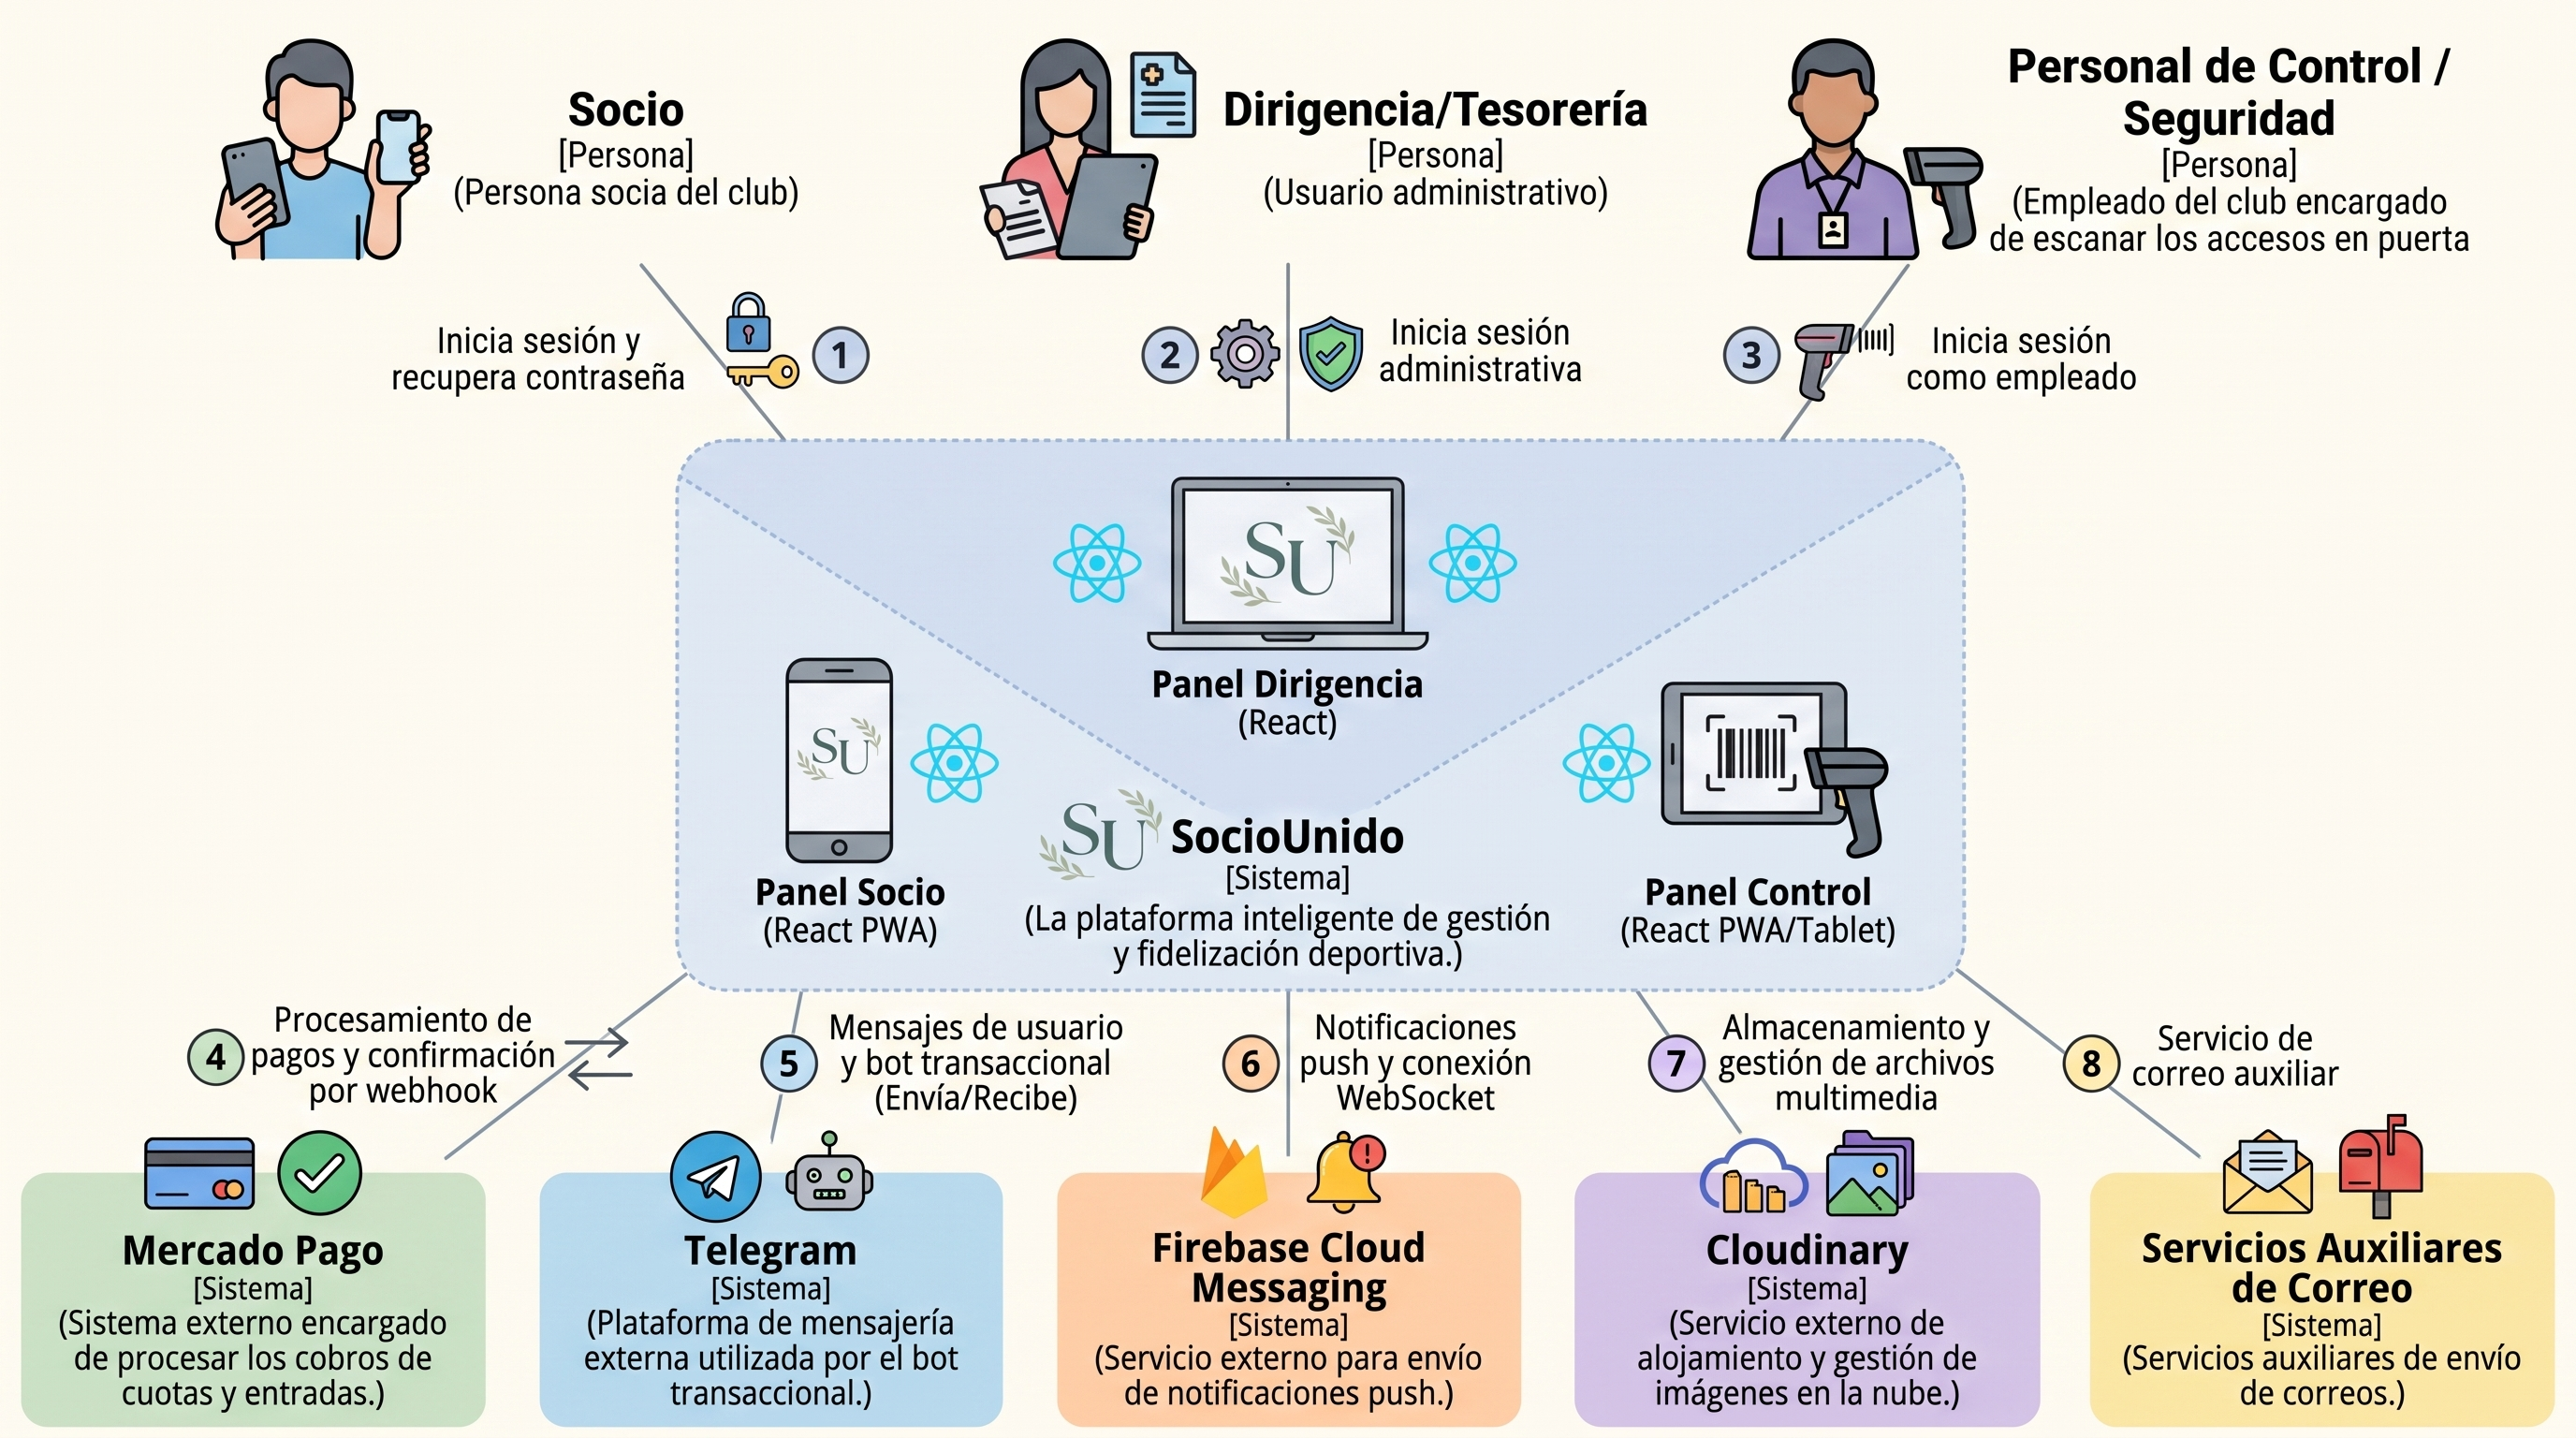
\includegraphics[width=\columnwidth]{img/arquitectura/c1_contexto.jpg}}
\caption{Diagrama de Contexto (C1) simplificado del ecosistema SocioUnido, ilustrando las fronteras de integraci\'on con actores humanos y servicios externos (Mercado Pago, Telegram, Cloudinary, Firebase).}
\label{fig:c1_contexto}
\end{figure}

\subsection{Automatizaci\'on de tareas mediante canalizaciones de integraci\'on y despliegue continuo (CI/CD)}
La velocidad de entrega y la estabilidad del ecosistema se garantizaron mediante la automatizaci\'on completa de los flujos de compilaci\'on, verificaci\'on y despliegue de \textit{software} utilizando la herramienta de automatizaci\'on integrada \textit{GitHub Actions}. La adopci\'on de esta tecnolog\'ia elimin\'o la necesidad de configurar servidores de automatizaci\'on externos complejos, ejecutando las tuber\'ias directamente sobre la infraestructura del proveedor de manera integrada con cada Pull Request.

Las canalizaciones l\'ogicas de integraci\'on continua (\textit{CI}) implementaron una estrategia de barreras de calidad autom\'aticas (\textit{Quality Gates}) que imped\'ian la fusi\'on de c\'odigo defectuoso a las ramas principales: al abrir un Pull Request, el flujo disparaba de forma autom\'atica las rutinas de formateo de c\'odigo, verificaba que no existieran fallos de sintaxis o empaquetado, ejecutaba la bater\'ia completa de pruebas unitarias as\'incronas con \textit{Pytest} y computaba el porcentaje de cobertura de c\'odigo (\textit{code coverage}). 

Solo si el c\'odigo fuente superaba con \'exito el 100\% de las pruebas de aserci\'on automatizadas y la cobertura de los tests se manten\'ia por encima del umbral fijado en el plan de calidad, la compuerta de integraci\'on habilitaba el bot\'on de fusi\'on para el responsable de \'area.

Una vez aprobada y fusionada la rama de desarrollo de forma as\'incrona, se activaban autom\'aticamente las canalizaciones de despliegue continuo (\textit{CD}) para actualizar en tiempo real los entornos productivos el\'asticos en la nube :
\begin{itemize}
    \item Las interfaces de usuario de \textit{frontend} se compilaban y alojaban de manera directa sobre la plataforma de computaci\'on el\'astica \textit{Vercel}, aprovechando su alta optimizaci\'on para aplicaciones React.
    \item Los componentes de \textit{backend} se empaquetaban en contenedores de infraestructura ligera mediante im\'agenes Docker y se desplegaban de manera ininterrumpida sobre la plataforma de servicios en la nube \textit{Render}.
\end{itemize}

\subsection{Inspecci\'on profunda y ciberseguridad continua: Dependabot y SonarCloud}
Para asegurar que SocioUnido se mantuviera en el estado del arte de la ciberseguridad y la ingenier\'ia de \textit{software}, el ciclo de vida de desarrollo incorpor\'o un enfoque proactivo de DevSecOps, integrando herramientas de an\'alisis est\'atico y de protecci\'on de cadena de suministro en cada repositorio de la organizaci\'on :

\begin{itemize}
    \item \textbf{Monitoreo continuo de dependencias (Dependabot)}: Al estar basados en lenguajes como Python y Node.js, los microservicios dependen de una amplia red de paquetes y librer\'ias de terceros susceptibles a brechas de seguridad y exposiciones p\'ublicas de vulnerabilidades (CVEs). Para neutralizar este riesgo de forma automatizada, se configur\'o Dependabot de manera transversal en todos los repositorios. La herramienta escanea ininterrumpidamente los manifiestos de dependencias, cruza los datos con bases de datos globales de vulnerabilidades actualizadas en tiempo real y, al detectar una brecha, genera de manera aut\'onoma un Pull Request con la actualizaci\'on exacta a la versi\'on segura m\'inima, garantizando la paridad con la suite de pruebas automatizadas del pipeline de CI antes de su fusi\'on.
    \item \textbf{An\'alisis est\'atico de c\'odigo estricto (SonarCloud)}: Mientras que Dependabot auditaba el c\'odigo de terceros, la calidad de la l\'ogica de negocio propia desarrollada por los estudiantes se someti\'o al an\'alisis est\'atico de caja blanca mediante la integraci\'on directa de SonarCloud como motor de SAST (Static Application Security Testing). En cada ejecuci\'on, SonarCloud analizaba la complejidad ciclom\'atica del c\'odigo, identificaba puntos propicios a fallos de desbordamiento, detectaba la presencia de c\'odigo muerto o duplicaciones, y auditaba la cobertura de c\'odigo de los Pull Requests. Los badges de control del estado de SonarCloud de cada microservicio se expusieron de manera din\'amica en el repositorio central \texttt{.github}, conformando una torre de control transparente y auditable que garantizaba que ninguna pieza de c\'odigo fuera integrada con deuda t\'ecnica acumulada.
\end{itemize}

\begin{figure}[htbp]
\centerline{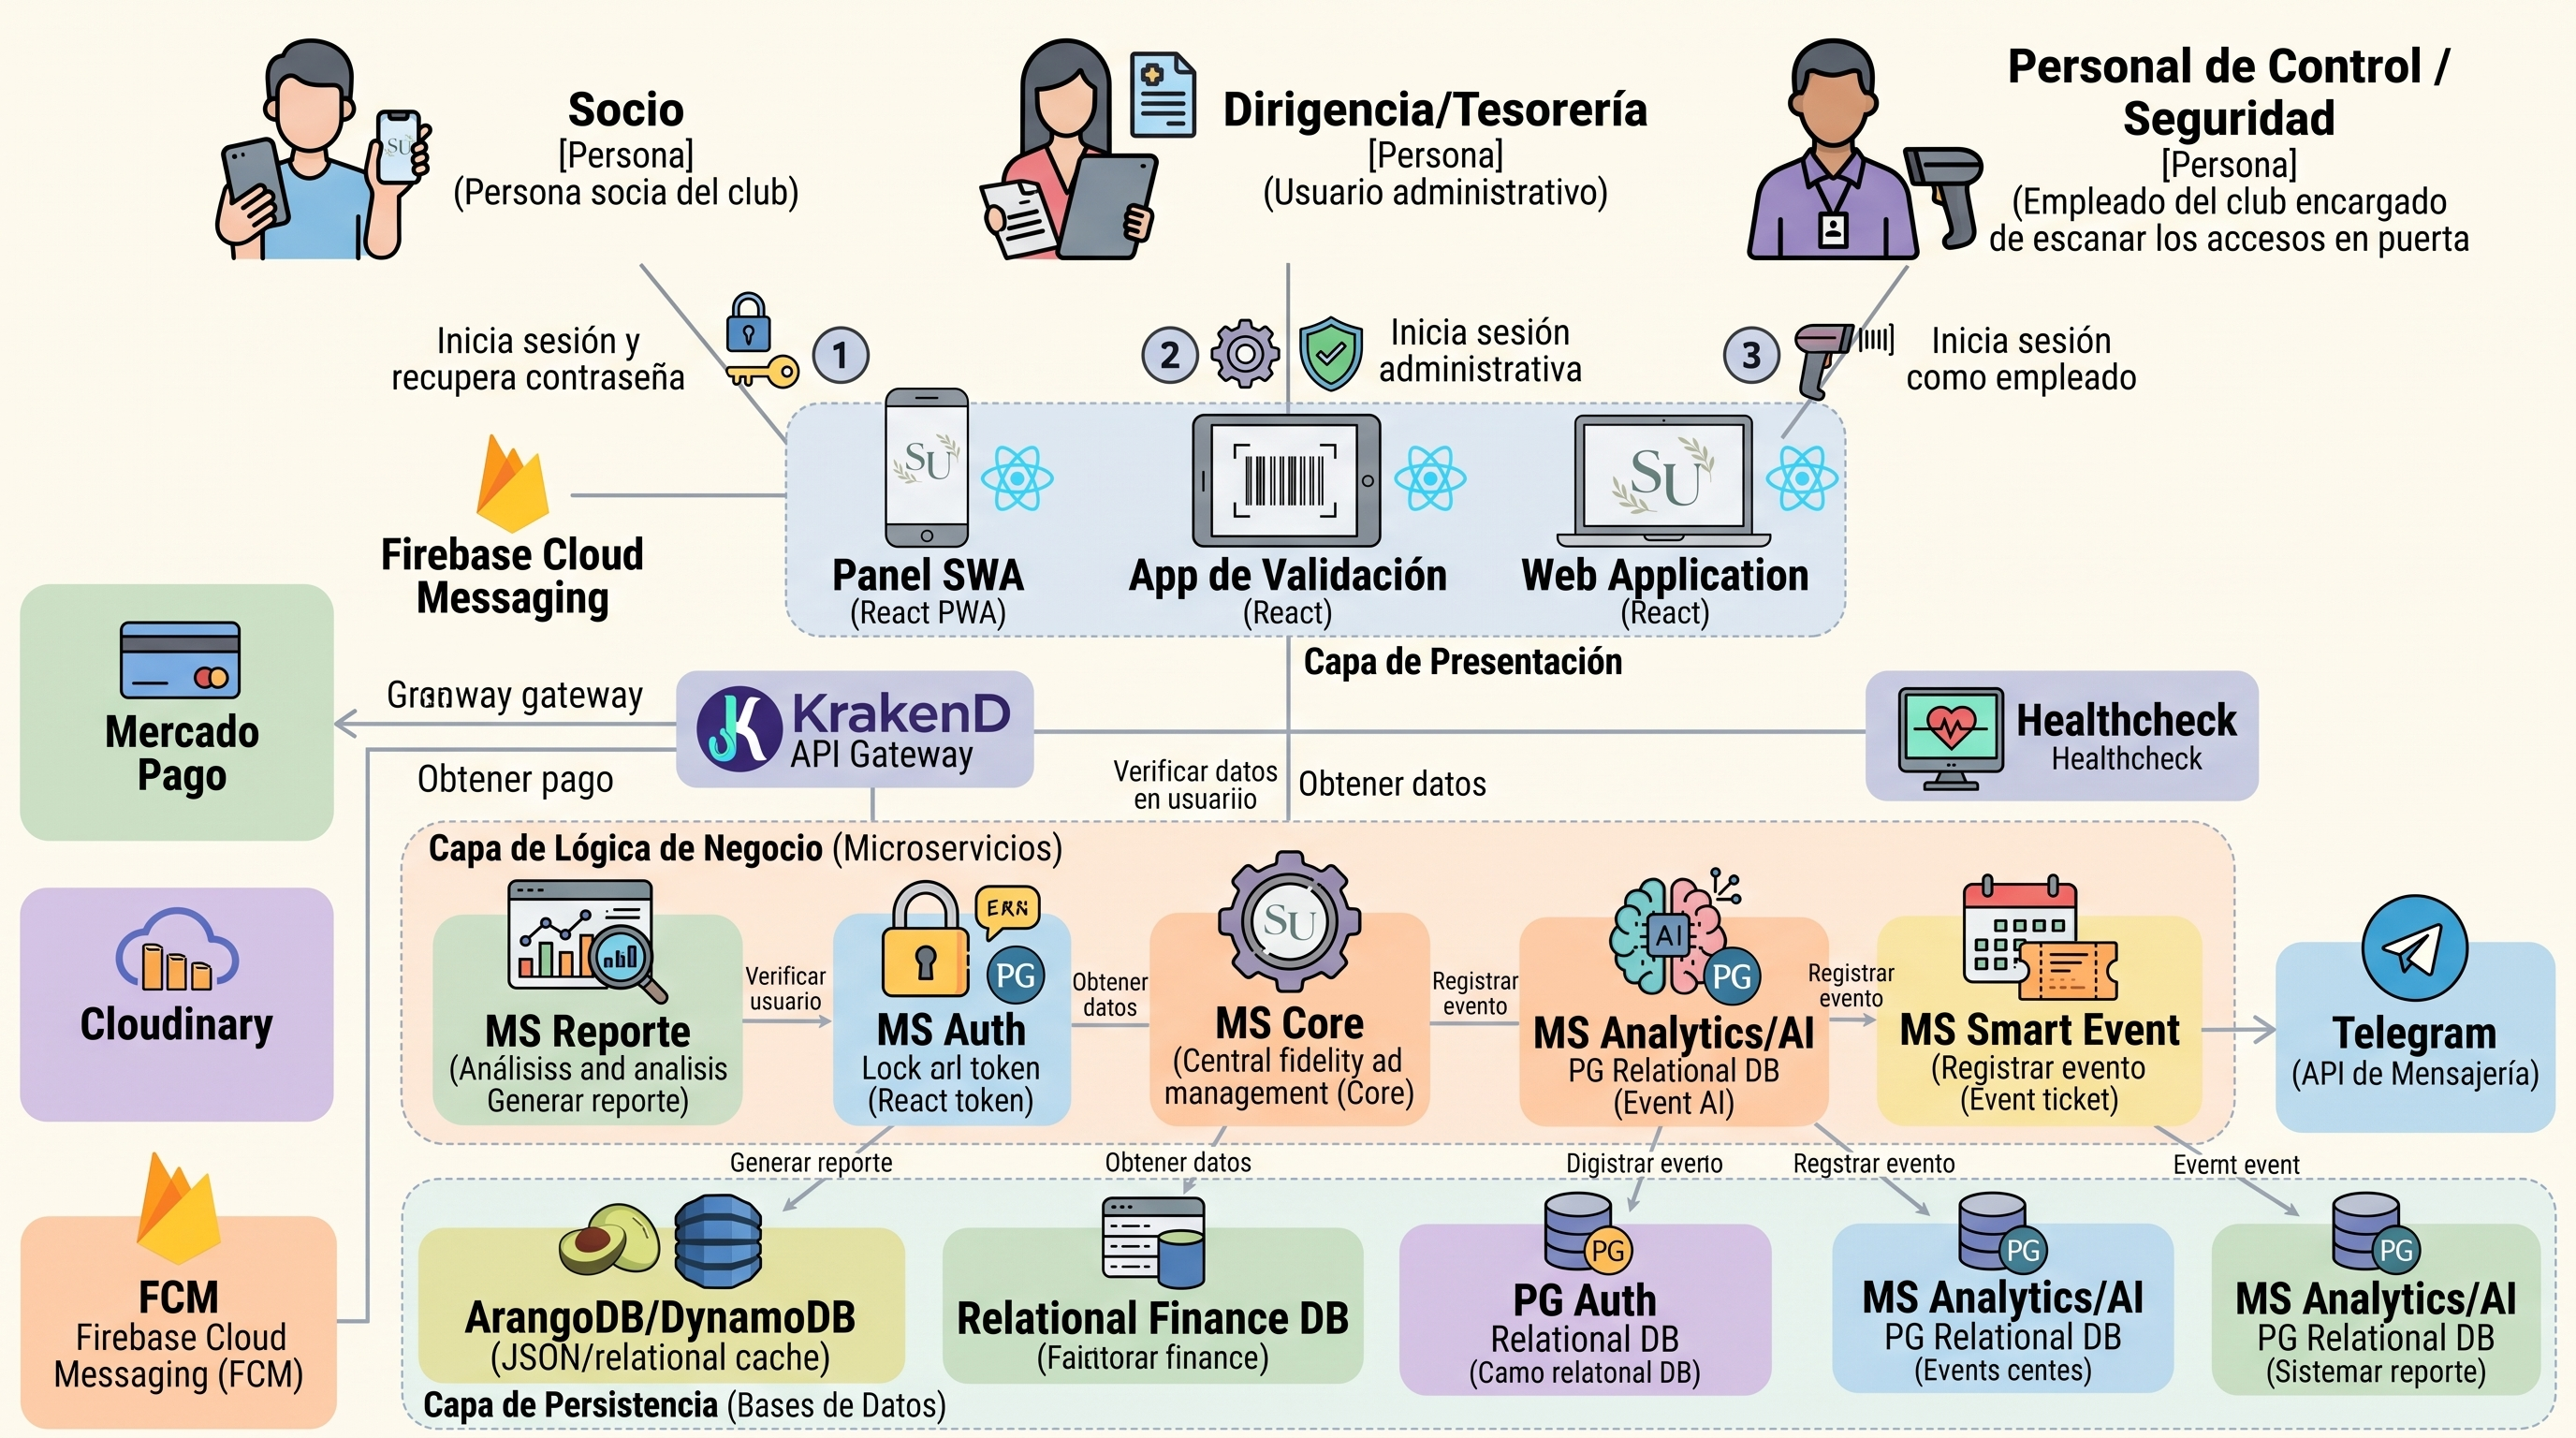
\includegraphics[width=\columnwidth]{img/arquitectura/c2_componentes.jpg}}
\caption{Diagrama de Contenedores (C2), detallando el aislamiento de las interfaces de \textit{frontend} respecto a la capa de l\'ogica de negocio (Microservicios en Python/FastAPI) y la capa de persistencia.}
\label{fig:c2_componentes}
\end{figure}

% ==========================================
\section{Experimentaci\'on, validaci\'on y control de calidad}
% ==========================================

Para garantizar la robustez, seguridad y fiabilidad de la plataforma \textbf{SocioUnido}, se ejecut\'o una estrategia integral de pruebas a lo largo de todo el ciclo de desarrollo. Este plan de validaci\'on certific\'o que el sistema cumple con la totalidad de los requerimientos funcionales y no funcionales especificados en las etapas tempranas del proyecto.

\subsection{Roles, responsabilidades y grado de automatizaci\'on}
La especificaci\'on, dise\~no y supervisi\'on del plan de pruebas estuvo a cargo del \textbf{Responsable de Control de Calidad (QA)}. Su rol consisti\'o en definir los casos de prueba, configurar los entornos de automatizaci\'on y ejecutar las pruebas manuales exploratorias. En concordancia con las pr\'acticas \'agiles, los desarrolladores de cada m\'odulo (\textit{front-end, back-end, IA}) fueron responsables de escribir y mantener las pruebas unitarias de su propia implementaci\'on.

La estrategia adopt\'o un enfoque de ``Pir\'amide de Pruebas'', priorizando un alto grado de automatizaci\'on en las capas inferiores para agilizar la Integraci\'on y Despliegue Continuo (CI/CD), reservando las pruebas manuales para la validaci\'on de usabilidad y flujos complejos:

\begin{itemize}
    \item \textbf{Pruebas unitarias (automatizadas):} Se valid\'o el correcto funcionamiento de funciones y m\'etodos aislados utilizando \textit{frameworks} est\'andar de la industria, integrados directamente en los repositorios.
    \item \textbf{Pruebas de integraci\'on (automatizadas):} Se verific\'o la correcta comunicaci\'on entre los microservicios, la base de datos relacional y las API de terceros (pasarelas de pago, Resend y Telegram).
    \item \textbf{Pruebas de extremo a extremo [End-to-End] (semiautomatizadas):} Se simularon flujos completos de usuario (por ejemplo, el pago de una cuota desde la PWA del socio hasta su reflejo en el panel de control administrativo).
\end{itemize}

\subsection{Validaci\'on funcional y no funcional}
El conjunto de pruebas funcionales se centr\'o en auditar los m\'odulos principales (\textit{core}) del ecosistema:

\begin{itemize}
    \item \textbf{Gesti\'on administrativa:} Verificaci\'on de los flujos de creaci\'on, lectura, actualizaci\'on y borrado (CRUD) del padr\'on de socios, y la correcta renderizaci\'on de m\'etricas.
    \item \textbf{Procesamiento de pagos:} Validaci\'on de la conciliaci\'on de pagos y webhooks con pasarelas externas.
    \item \textbf{Asistente conversacional (PLN):} Pruebas de caja negra sobre el bot de Telegram (``BotIn''), inyectando frases de intenci\'on variada (texto formal, informal, modismos) para validar la precisi\'on del reconocimiento de lenguaje natural.
    \item \textbf{Acceso inteligente [Smart Access] (TOTP):} Comprobaci\'on rigurosa del algoritmo criptogr\'afico y evaluaci\'on de la correctitud de su funcionamiento offline.
\end{itemize}

A nivel no funcional, la plataforma fue sometida a pruebas de rendimiento simulando picos extremos de tr\'afico para asegurar la estabilidad durante los d\'ias de partido. Asimismo, se verific\'o la compatibilidad multiplataforma de las interfaces web y m\'oviles, y se audit\'o el cifrado de datos en reposo y en tr\'ansito.

\subsection{Validaci\'on con usuarios finales y UX/UI}
Considerando que la usabilidad y la adecuaci\'on al mercado son pilares vitales para la adopci\'on masiva del sistema, se ejecut\'o una etapa de validaci\'on participativa orientada a medir la satisfacci\'on real de los usuarios. Que al hincha le resulte intuitiva la aplicaci\'on y al trabajador del club le aporte soluciones pr\'acticas son factores cr\'iticos de \'exito.

\begin{itemize}
    \item \textbf{Validaci\'on de producto con clubes:} Se llevaron a cabo reuniones con personal administrativo y directivo de diferentes instituciones para presentarles el producto y exponer sus valores agregados. El objetivo central de estos encuentros fue obtener \textit{feedback} directo sobre la utilidad real de la soluci\'on, relevar puntos de mejora y analizar las principales diferencias competitivas de SocioUnido frente a las plataformas de gesti\'on preexistentes en el mercado.
    \item \textbf{Validaci\'on masiva mediante Google Forms:} Se distribuyeron encuestas estructuradas a una muestra significativa de socios finales (\textit{beta-testers}) luego de que interactuaran con la aplicaci\'on m\'ovil (PWA). Este formulario recolect\'o m\'etricas precisas sobre la intuici\'on del dise\~no, la usabilidad y la fluidez de los procesos dentro de la aplicaci\'on. El \textit{feedback} obtenido fue un insumo cr\'itico que permiti\'o refinar la interfaz y garantizar una experiencia de usuario (UX/UI) de alt\'isima calidad antes del despliegue final.
\end{itemize}

\subsection{QA automatizado con agente de OpenClaw}
En el marco del desarrollo de SocioUnido, alcanzar la m\'as alta calidad en los est\'andares de ciberseguridad y de interoperabilidad se plante\'o como un objetivo innegociable. Para que el ecosistema se mantenga a la vanguardia, resulta clave que la arquitectura y los \textit{endpoints} est\'en preparados no solo para usuarios humanos, sino tambi\'en para integrarse de manera fluida y segura con agentes aut\'onomos de terceros e Inteligencias Artificiales.

Para llevar a cabo una validaci\'on rigurosa, se implement\'o \textbf{OpenClaw}, un agente de IA dise\~nado espec\'ificamente para el \textit{testing} automatizado y el QA integral de repositorios. Su adopci\'on se justifica por su capacidad para comprender el contexto del c\'odigo e identificar vulnerabilidades l\'ogicas complejas.

\subsubsection{Directrices del agente}
La implementaci\'on t\'ecnica del agente se bas\'o en un marco de instrucciones precisas (\textit{prompting}) que auditan estrictamente tres ejes fundamentales:
\begin{itemize}
    \item \textbf{Seguridad de la implementaci\'on:} B\'usqueda exhaustiva de vulnerabilidades, haciendo foco en los est\'andares de la industria (OWASP Top 10) y prevenci\'on de vectores de ataque.
    \item \textbf{Prevenci\'on de fuga de datos:} Asegurar rigurosamente que el c\'odigo fuente no exponga credenciales, tokens de acceso ni informaci\'on privada de los usuarios.
    \item \textbf{Preparaci\'on para IA y automatizaci\'on:} Evaluar si la estructura de los datos est\'a dise\~nada para garantizar una interacci\'on sin fricciones con futuras automatizaciones.
\end{itemize}

\subsubsection{Resultados obtenidos}
A continuaci\'on, se detalla el an\'alisis exhaustivo de seguridad realizado por OpenClaw sobre los repositorios principales que conforman la arquitectura de SocioUnido.

\noindent \textbf{Aplicaci\'on m\'ovil PWA (Socios)}
\begin{itemize}
    \item \textbf{Fuga de informaci\'on sensible:} Se identific\'o que, ante fallos inesperados, el componente capturador de errores expon\'ia la traza completa del sistema (\textit{stack trace}) en pantalla.
    \item \textbf{Manipulaci\'on de rutas API:} Se detect\'o una concatenaci\'on directa e insegura de par\'ametros en peticiones HTTP, dejando abierta la posibilidad de alterar rutas (\textit{Path Traversal}).
    \item \textbf{Gesti\'on de encabezados de autorizaci\'on:} El m\'odulo de peticiones enviaba encabezados con valores nulos al navegar de forma an\'onima.
    \item \textbf{Exposici\'on de datos y tokens:} El contexto global registraba en consola informaci\'on personal y tokens de notificaciones.
    \item \textbf{Metadatos de idioma en documentos que confunden a agentes de IA.}
\end{itemize}

\noindent \textbf{Aplicaci\'on m\'ovil PWA (Trabajadores)}
\begin{itemize}
    \item \textbf{Fuga de informaci\'on sensible:} Exposici\'on de la traza completa del sistema en pantalla ante fallos.
    \item \textbf{Gesti\'on de encabezados:} Env\'io de encabezados nulos en navegaci\'on an\'onima.
    \item \textbf{Pol\'iticas de seguridad inexistentes:} Carencia de pol\'iticas de restricci\'on de contenido.
\end{itemize}

\noindent \textbf{API Gateway}
\begin{itemize}
    \item \textbf{Elevaci\'on de privilegios:} M\'odulos sensibles carec\'ian de verificaci\'on de permisos.
    \item \textbf{Ausencia de l\'imites de tr\'afico:} Rutas sin restricci\'on de peticiones por minuto.
    \item \textbf{Privilegios m\'aximos en contenedores:} Ejecuci\'on del servicio bajo el usuario \texttt{root}.
    \item \textbf{Desactivaci\'on de validaci\'on de llaves:} Descarga insegura de llaves criptogr\'aficas.
\end{itemize}

\noindent \textbf{Microservicio de accesos}
\begin{itemize}
    \item \textbf{Almacenamiento en texto plano:} Las semillas secretas para los c\'odigos din\'amicos (TOTP) se almacenaban sin cifrado.
    \item \textbf{Fuga de tokens en registros.}
    \item \textbf{Valores predeterminados r\'igidos.}
    \item \textbf{Pol\'iticas de origen cruzado ausentes.}
\end{itemize}

\noindent \textbf{Microservicio de anal\'iticas}
\begin{itemize}
    \item \textbf{Procesamiento deficiente de mensajes:} Lectura as\'incrona sin validaci\'on de estructura.
    \item \textbf{Autenticaci\'on vulnerable (Timing Attack):} Verificaci\'on de tokens mediante comparaciones de texto convencionales.
    \item \textbf{Contratos de interfaz incompletos.}
\end{itemize}

\noindent \textbf{Microservicio de autenticaci\'on}
\begin{itemize}
    \item \textbf{Pol\'iticas de contrase\~nas laxas:} Permisividad de claves demasiado cortas en el registro.
    \item \textbf{Estructuras gen\'ericas:} Uso de diccionarios sin tipo, impidiendo esquemas claros para IA.
\end{itemize}

\noindent \textbf{Microservicio de bot conversacional (PLN)}
\begin{itemize}
    \item \textbf{Falta de validaci\'on de firmas:} Ausencia de verificaci\'on criptogr\'afica de las peticiones del proveedor (Telegram/Meta).
    \item \textbf{Exposici\'on de datos en servidor:} Registros en consola de mensajes.
    \item \textbf{Ca\'idas por datos invalidos:} Excepciones cr\'iticas ante mensajes con formatos inesperados.
\end{itemize}

\noindent \textbf{Microservicio de gesti\'on del club (Core)}
\begin{itemize}
    \item \textbf{Exposici\'on de arquitectura interna:} Devoluci\'on de errores crudos revelando la estructura de las tablas de la base de datos.
    \item \textbf{Inconsistencia en contratos de datos:} M\'ultiples salidas de informaci\'on con fallas de validaci\'on de esquemas.
\end{itemize}

\noindent \textbf{Microservicio de pagos}
\begin{itemize}
    \item \textbf{Omisi\'on de autenticaci\'on en cobros:} Punto de acceso principal sin validaci\'on de clave interna.
    \item \textbf{Ausencia de verificaci\'on en webhooks:} Falta de validaci\'on de la firma criptogr\'afica.
    \item \textbf{Inseguridad en intermediario de eventos:} Conexi\'on a Redis con validaci\'on SSL/TLS.
    \item \textbf{Gesti\'on de credenciales:} Claves secretas d\'ebiles y expuestas en archivos de migraci\'on.
\end{itemize}

\noindent \textbf{Panel administrativo web}
\begin{itemize}
    \item \textbf{Exposici\'on de credenciales.}
    \item \textbf{Sobrecarga de memoria:} Descarga del padr\'on completo de socios sin paginaci\'on.
    \item \textbf{Vulnerabilidad XSS:} Inyecci\'on de enlaces e im\'agenes sin sanitizaci\'on previa.
    \item \textbf{Manipulaci\'on de rutas (Path Traversal):} Identificadores din\'amicos no codificados.
\end{itemize}

\subsubsection{Acciones tomadas y refactorizaci\'on}
Las observaciones del agente automatizado impulsaron una refactorizaci\'on integral en todos los m\'odulos de la aplicaci\'on:

\begin{itemize}
    \item \textbf{Cifrado y credenciales:} Se eliminaron contrase\~nas por defecto y claves en el c\'odigo, cifrando las semillas TOTP con algoritmos sim\'etricos.
    \item \textbf{Auditor\'ia de dependencias:} Se exigieron librer\'ias certificadas para mitigar ataques a la cadena de suministro.
    \item \textbf{Sanitizaci\'on y paginaci\'on:} Se aplicaron pol\'iticas CSP, codificaci\'on de par\'ametros y paginaci\'on del lado del servidor, previniendo fugas masivas de datos.
    \item \textbf{Concurrencia y privilegios:} Se integraron bloqueos de hilos en servicios compartidos y se aislaron los contenedores ejecut\'andolos sin privilegios administrativos (\texttt{root}).
    \item \textbf{Protecci\'on criptogr\'afica:} Se adoptaron comparaciones de tiempo constante (mitigando \textit{Timing Attacks}) y se forz\'o la validaci\'on de firmas en \textit{webhooks}.
    \item \textbf{Contratos para IA:} Se tiparon estrictamente los esquemas, estandarizando las respuestas de error para no revelar la arquitectura interna.
\end{itemize}

En conclusi\'on, las exhaustivas auditor\'ias de OpenClaw y sus posteriores correcciones dotaron a SocioUnido de una infraestructura robusta, cibersegura y preparada para integrarse sin fricciones con futuras plataformas y agentes inteligentes.

% ==========================================
\section{Conclusiones}
% ==========================================

Las conclusiones de este documento recapitulan los aspectos centrales descritos en las secciones anteriores, evaluando el alcance funcional del Producto M\'inimo Viable (MVP) entregado, el ecosistema documental construido y el impacto real de la plataforma. Esta visi\'on hol\'istica permite dimensionar el verdadero profesionalismo del proyecto y c\'omo este materializa la formaci\'on integral recibida a lo largo de la carrera.

\subsection{Resultados principales: Ecosistema organizativo y repositorios}
Absolutamente toda la implementaci\'on t\'ecnica, l\'ogica y documental del Trabajo Profesional reside de forma centralizada en nuestra organizaci\'on oficial de GitHub. La magnitud del proyecto exigi\'o una arquitectura sumamente distribuida, componi\'endose de \textbf{27 repositorios y 2 proyectos Kanban}.

\subsubsection{Gesti\'on \'agil y control de incidencias (Proyectos Kanban)}
\begin{itemize}
    \item \textbf{Centro de monitoreo de tareas:} Tablero estructurado bajo la metodolog\'ia Kanban que rigi\'o la ejecuci\'on de los 13 \textit{sprints} de desarrollo. Permiti\'o gestionar el \textit{backlog} de manera din\'amica, asignando responsables, pesos (esfuerzo) y prioridades a cada historia de usuario.
    \item \textbf{Centro de monitoreo de bugs:} Espacio hom\'ologo dedicado exclusivamente a la detecci\'on, seguimiento y resoluci\'on de errores (\textit{bugs}) y deudas t\'ecnicas reportadas por los auditores autom\'aticos (SonarCloud/OpenClaw).
\end{itemize}

\subsubsection{Repositorios privados (L\'ogica de negocio e infraestructura)}
Con el fin de resguardar la propiedad intelectual, la seguridad criptogr\'afica y los derechos de autor de las implementaciones subyacentes, los repositorios \textit{back-end} se mantienen en car\'acter privado. Sin embargo, \textbf{ante cualquier requerimiento acad\'emico, de evaluaci\'on o inter\'es t\'ecnico justificado, el equipo est\'a totalmente a disposici\'on para otorgar los accesos correspondientes}. El c\'odigo fuente de estos repositorios est\'a documentado internamente siguiendo los m\'as altos est\'andares y buenas pr\'acticas (\textit{self-documenting code}).

\subsubsection{Repositorios p\'ublicos (Interfaces y portales documentales)}
La totalidad de las interfaces cliente y la documentaci\'on asociada a los repositorios privados se mantienen en car\'acter p\'ublico para demostrar la transparencia, alcance y arquitectura del proyecto sin comprometer credenciales sensibles.

\textbf{Portales documentales de la arquitectura (\textit{Back-end}):} Para cada microservicio privado existe un repositorio espejo terminado en \texttt{-doc}. Estos alojan portales generados con JustTheDocs que explican exhaustivamente la arquitectura del servicio original: diagramas de contexto, justificaci\'on tecnol\'ogica, m\'etricas de implementaci\'on y el listado de \textit{endpoints} p\'ublicos.

\textbf{Interfaces gr\'aficas (\textit{Front-end}):} Exponen el c\'odigo y sus propias p\'aginas documentales con vistas principales del sistema (\texttt{plataforma-web}, \texttt{aplicacion}, \texttt{control-de-accesos}).

\subsection{El inmenso valor documental del proyecto}
El hito m\'as destacable de SocioUnido, a la par de su alcance tecnol\'ogico, es su aporte documental. Se han construido \textbf{16 p\'aginas plenamente documentales con JustTheDocs} que abarcan el Trabajo Profesional de punta a punta (8 de arquitectura, 3 visuales y 5 de gesti\'on global). Particularmente, el repositorio \texttt{documentacion} aloja una vasta cantidad de material complementario:

\begin{itemize}
    \item El Anteproyecto y las versiones iterativas de la Entrega Intermedia.
    \item Evidencia de validaci\'on del producto (entrevistas a trabajadores y encuestas de usabilidad).
    \item El Informe Final definitivo y diagramas del Modelo C4 / DER.
    \item Redacciones de discursos comerciales (\textit{Pitch}) y desarrollo de identidad visual de marca.
    \item M\'as de \textbf{25 anexos formales} analizando aristas t\'ecnicas, legales y de gesti\'on.
    \item Decenas de videotutoriales explicativos de la plataforma con sus manuales de uso.
\end{itemize}

\subsection{Identidad comercial, innovaci\'on y contribuci\'on a otras entidades}
Desde su concepci\'on, SocioUnido fue tratado como un producto real. Para respaldar esta visi\'on, se consolid\'o una \textbf{P\'agina publicitaria (Landing Page)} y un \textbf{Canal de YouTube} para validaci\'on y tutoriales. Este enfoque comercial fue validado de forma emp\'irica y constante mediante reuniones con trabajadores de clubes reales y encuestas a usuarios finales.

A partir de este desarrollo, el Trabajo Profesional ha generado \textbf{innovaciones tecnol\'ogicas} significativas que contribuyen directamente a la modernizaci\'on, inclusi\'on y saneamiento de las instituciones deportivas (especialmente en las categor\'ias de ascenso):
\begin{enumerate}
    \item \textbf{Innovaci\'on criptogr\'afica (Infraestructura \textit{offline}):} Adaptaci\'on del algoritmo TOTP para la validaci\'on de accesos en estadios sin conexi\'on a internet, mitigando el colapso de las redes 4G/5G en eventos masivos y erradicando el fraude sin requerir hardware costoso.
    \item \textbf{Innovaci\'on predictiva:} Desarrollo de herramientas para predecir el riesgo de fuga societaria bas\'andose en historiales y m\'etricas definidas por el club, transformando la cobranza reactiva en un modelo de retenci\'on proactiva.
    \item \textbf{Innovaci\'on en accesibilidad (PLN):} Democratizaci\'on del sistema mediante un asistente omnicanal en Telegram con Procesamiento de Lenguaje Natural, eliminando la fricci\'on tecnol\'ogica para usuarios de todas las edades.
\end{enumerate}

\subsection{Impacto en la formaci\'on: Conocimientos aplicados}
El dise\~no, arquitectura y desarrollo de la plataforma SocioUnido no es un esfuerzo aislado, sino la s\'intesis y aplicaci\'on directa de los conocimientos adquiridos a lo largo de toda la carrera de Ingenier\'ia en Inform\'atica. La resoluci\'on de las problem\'aticas de las instituciones deportivas exigi\'o un enfoque multidisciplinario:

\begin{itemize}
    \item \textbf{Fundamentos matem\'aticos, ciencias b\'asicas y algoritmos:} \textit{F\'isica} provey\'o el conocimiento sobre la propagaci\'on de se\~nales, justificando la validaci\'on de ingresos de forma \textit{offline} en estadios repletos. \textit{\'Algebra A y \'Algebra Lineal} fueron indispensables para comprender la criptograf\'ia (aritm\'etica modular y \textit{hash}) detr\'as de la innovaci\'on TOTP. \textit{Qu\'imica} aport\'o la perspectiva de las limitaciones de las bater\'ias de los dispositivos de escaneo m\'ovil a la intemperie. \textit{Algoritmos y Estructuras de Datos, y Teor\'ia de Algoritmos} constituyeron el n\'ucleo de eficiencia, optimizando las b\'usquedas y el filtrado de enormes padrones. Finalmente, \textit{An\'alisis Matem\'atico y Probabilidad y Estad\'istica} aportaron el marco te\'orico para la evaluaci\'on y limpieza de datos.
    \item \textbf{Ingenier\'ia de software, arquitectura y calidad:} \textit{Ingenier\'ia de Software I y II} guiaron la concepci\'on del ciclo de vida, la aplicaci\'on de Scrum, arquitecturas de microservicios (alta cohesi\'on y bajo acoplamiento) y el \textit{Delivery Pipeline} (CI/CD). Materias como \textit{Taller de Programaci\'on y Paradigmas de Programaci\'on} forjaron las bases de pruebas automatizadas (TDD) y el desarrollo de c\'odigo limpio y escalable.
    \item \textbf{Sistemas, redes y bases de datos:} \textit{Organizaci\'on del Computador y Sistemas Operativos} permitieron comprender la arquitectura a bajo nivel y el manejo de memoria en contenedores. \textit{Base de Datos} asegur\'o la persistencia y normalizaci\'on mediante transacciones concurrentes en PostgreSQL. \textit{Programaci\'on Concurrente, Redes y Sistemas Distribuidos I} resultaron la columna vertebral de la plataforma Cloud, garantizando balanceo de carga, protocolos de red (HTTP/TCP), APIs RESTful y tolerancia a fallos.
    \item \textbf{Ciencia de datos y Ciberseguridad:} Los conocimientos de \textit{Ciencia de Datos} sirvieron para procesar grandes vol\'umenes de transacciones y extraer caracter\'isticas proyectando soluciones de retenci\'on. En paralelo, el \textit{Taller de Seguridad Inform\'atica} aport\'o las t\'ecnicas de defensa en profundidad, sanitizaci\'on de datos y gesti\'on de roles (JWT) para proteger la informaci\'on.
    \item \textbf{Emprendedurismo, gesti\'on y contexto profesional:} \textit{Introducci\'on al Conocimiento de la Sociedad y el Estado e Introducci\'on al Pensamiento Cient\'ifico} brindaron el pensamiento cr\'itico para entender la din\'amica sociopol\'itica de los clubes. \textit{Empresas de Base Tecnol\'ogica I y II} sentaron las bases corporativas, financieras y legales del modelo SaaS B2B, estrategias de \textit{pricing} y propiedad intelectual. Por \'ultimo, \textit{Gesti\'on del Desarrollo de Sistemas Inform\'aticos} aport\'o la estructura ejecutiva para estimar tiempos, liderar al equipo y gestionar los riesgos del proyecto.
\end{itemize}

\subsection{Cierre y reflexi\'on final}
En s\'intesis, SocioUnido no es un mero ensamblaje de tecnolog\'ias, sino el producto maduro de un ingeniero inform\'atico formado integralmente en la Universidad de Buenos Aires (UBA), capaz de integrar ciencias b\'asicas, aplicadas, y competencias de gesti\'on para resolver problemas complejos de la sociedad y la industria.

El c\'odigo fuente en su totalidad cuenta con m\'as de \textbf{1.200} \textit{commits} registrados y \textbf{290} revisiones cruzadas (\textit{Pull Requests}) evaluadas. El volumen estructural desarrollado impact\'o en aproximadamente \textbf{400.000} l\'ineas de c\'odigo a lo largo de este a\~no de desarrollo continuo.

Por esto, y por el impacto real del producto construido, el equipo no podr\'ia estar m\'as orgulloso de los resultados obtenidos. Tenemos la profunda convicci\'on de que el Trabajo Profesional que estamos entregando representa el m\'as alto est\'andar de excelencia institucional. Haber fortalecido el proyecto en todos los aspectos evaluables (tecnol\'ogicos, comerciales, documentales y arquitect\'onicos) demuestra que el trayecto formativo de nuestra carrera ha rendido sus frutos, cerrando esta etapa universitaria con un broche de oro materializado en este impresionante entregable final.

% ==========================================
\section{Referencias}
% ==========================================

\begin{thebibliography}{00}

\bibitem{anthropic} Anthropic. (s.f.). \textit{Claude Documentation}. Recuperado de \url{https://docs.anthropic.com/}

\bibitem{cloudinary} Cloudinary. (s.f.). \textit{Cloudinary Documentation}. Recuperado de \url{https://cloudinary.com/documentation}

\bibitem{fiuba} Consejo Directivo, Facultad de Ingenier\'ia, Universidad de Buenos Aires. (22 de diciembre de 2025). \textit{Resoluci\'on N$^\circ$ RESCD-2025-1124-E-UBA-DCT\_FI: Reglamento de Trabajo Integrador Final para carreras de grado FIUBA}. Recuperado de \url{https://cms.fi.uba.ar/uploads/RESCD_2025_1124_Reglamento_de_Trabajo_Integrador_Final_para_carreras_de_grado_6da340c642.pdf}

\bibitem{docker} Docker Inc. (s.f.). \textit{Docker Documentation}. Recuperado de \url{https://docs.docker.com/}

\bibitem{figma} Figma. (s.f.). \textit{Figma Help Center}. Recuperado de \url{https://help.figma.com/}

\bibitem{github} GitHub. (s.f.). \textit{GitHub Docs (incluye GitHub Actions y Dependabot)}. Recuperado de \url{https://docs.github.com/}

\bibitem{globalfan} Global.fan. (s.f.). \textit{Global.fan - Plataforma de gesti\'on deportiva y engagement}. Recuperado de \url{https://global.fan}

\bibitem{firebase} Google. (s.f.). \textit{Firebase Documentation}. Recuperado de \url{https://firebase.google.com/docs}

\bibitem{gemini} Google. (s.f.). \textit{Gemini AI}. Recuperado de \url{https://deepmind.google/technologies/gemini/}

\bibitem{krakend} KrakenD. (s.f.). \textit{KrakenD API Gateway Documentation}. Recuperado de \url{https://www.krakend.io/docs/}

\bibitem{mercadopago} Mercado Pago. (s.f.). \textit{Mercado Pago Developers}. Recuperado de \url{https://www.mercadopago.com.ar/developers/es/docs}

\bibitem{react} Meta Platforms, Inc. (s.f.). \textit{React Documentation}. Recuperado de \url{https://react.dev/}

\bibitem{neon} Neon. (s.f.). \textit{Neon Serverless Postgres Documentation}. Recuperado de \url{https://neon.tech/docs/}

\bibitem{openai} OpenAI. (s.f.). \textit{OpenAI Documentation}. Recuperado de \url{https://platform.openai.com/docs/}

\bibitem{python} Python Software Foundation. (s.f.). \textit{Python 3 Documentation}. Recuperado de \url{https://docs.python.org/3/}

\bibitem{redis} Redis. (s.f.). \textit{Redis Documentation}. Recuperado de \url{https://redis.io/docs/}

\bibitem{render} Render. (s.f.). \textit{Render Documentation}. Recuperado de \url{https://render.com/docs}

\bibitem{resend} Resend. (s.f.). \textit{Resend Documentation}. Recuperado de \url{https://resend.com/docs}

\bibitem{sonarcloud} SonarSource. (s.f.). \textit{SonarCloud Documentation}. Recuperado de \url{https://docs.sonarsource.com/sonarcloud/}

\bibitem{sqlalchemy} SQLAlchemy. (s.f.). \textit{SQLAlchemy Documentation}. Recuperado de \url{https://docs.sqlalchemy.org/}

\bibitem{telegram} Telegram. (s.f.). \textit{Telegram Bot API}. Recuperado de \url{https://core.telegram.org/bots/api}

\bibitem{fastapi} Tiangolo. (s.f.). \textit{FastAPI Documentation}. Recuperado de \url{https://fastapi.tiangolo.com/}

\bibitem{tn} Todo Noticias (TN). (28 de enero de 2026). \textit{La AFA revel\'o cu\'antos socios tienen los clubes de Primera Divisi\'on: c\'omo qued\'o el ranking}. Recuperado de \url{https://tn.com.ar/deportes/futbol/2026/01/28/la-afa-revelo-cuantos-socios-tienen-los-clubes-de-primera-division-como-quedo-el-ranking/}

\bibitem{vercel} Vercel. (s.f.). \textit{Vercel Documentation}. Recuperado de \url{https://vercel.com/docs}

\bibitem{vite} Vite. (s.f.). \textit{Vite Documentation}. Recuperado de \url{https://vitejs.dev/}

\end{thebibliography}

\end{document}
